\documentclass{scrartcl}

\usepackage{ucs}
\usepackage[utf8x]{inputenc}
\usepackage[ngerman]{babel}
\usepackage{graphicx}
\usepackage{amsmath}
\usepackage{amssymb}
\usepackage{color}
\usepackage{grffile}

\title{Virtuelle Maschinen \\ Zusammenfassung}
\author{Thomas Mohr}
\date{}

\begin{document}
\maketitle

\section{Introduction}

\subsection{Standard Interfaces}

\subsubsection{Advantages}

\begin{itemize}
	\item Major design tasks are decoupled (in space and time)
	\item Different hardware and software development schedules
	\item Software can run on any machine supporting a compatible interface \\
	
	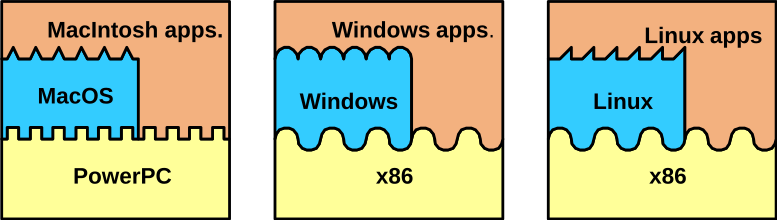
\includegraphics[width=0.8\textwidth]{figures/StandardInterfacesAdvantages.png}
\end{itemize}

\subsubsection{Disadvantages}

\begin{itemize}
	\item Software compiled for one Industry Standard Architecture (ISA) will not run on hardware with a different ISA \\
	
	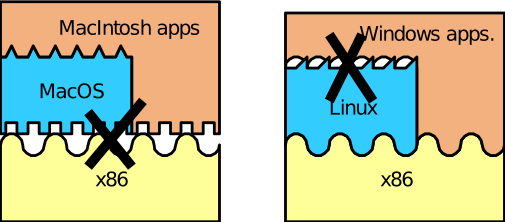
\includegraphics[width=.6\textwidth]{figures/StandardInterfacesDisadvantages.png}
	\item Binary may not be optimzed for the specific hardware platform it runs on
	\item Innovation may be inhibited by fixed ISA
	\begin{itemize}
		\item Hard to add new or remove obsolete instrcutions
	\end{itemize}
	\item Difficult for software to interact directly with implementation
	\begin{itemize}
		\item Performance features
		\item Power management
		\item Fault tolerance
		\item Software is supposed to be implementation independant
	\end{itemize}
\end{itemize}

\subsection{Hardware Resources}

\begin{itemize}
	\item Conventional system software manages hardware resources directly
	\begin{itemize}
		\item An operating System (OS) manages the physical memory of a specific size
		\item Input/Output (I/O) devices are managed as physical entities
	\end{itemize}
	\item Difficult to share resources except through OS
	\begin{itemize}
		\item All users of hardware must use the same OS
		\item All users are vulnerable to attacks from other users sharing the resource (via security holes in the OS)
	\end{itemize}
\end{itemize}

\subsection{Abstraction}

\begin{itemize}
	\item Computer systems are built on levels of abstraction
	\begin{itemize}
		\item Higher levels of abstraction hide details at lower levels
		\item Example: Files are an abstraction of a disk \\
		
		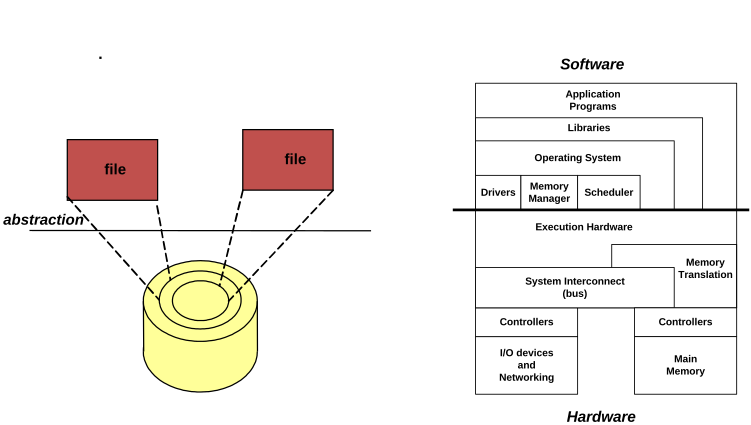
\includegraphics[width=.8\textwidth]{figures/Abstraction.png}
	\end{itemize}
\end{itemize}

\subsection{Virtualization}

\begin{itemize}
	\item An isomorphism from guest to host
	\begin{itemize}
		\item Map guest state to host state
		\item Implement ''equivalent'' functions
	\end{itemize}
	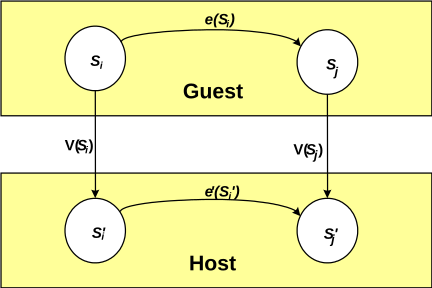
\includegraphics[width=.5\textwidth]{figures/VirtualizationGuestHost.png}
	\item Similar to abstraction (details are not necessarily hidden)
	\item Constrcut Virtual Disks
	\begin{itemize}
		\item As files on a larger disk
		\item Map state
		\item Implement functions
	\end{itemize}
	\item Virtual machines (VM) do the same thing with the whole ''machine'' \\
	
	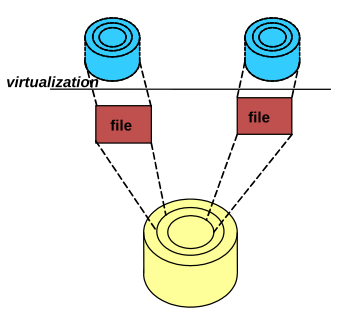
\includegraphics[width=0.5\textwidth]{figures/VirtualizationVirtualDisks.png}
\end{itemize}

\subsection{The ''Machine''}

\begin{itemize}
	\item Different perspectives on what the ''Machine'' is:
	\begin{itemize}
		\item OS developer
		\begin{itemize}
			\item ISA
			\item Major division between hardware and software
		\end{itemize}
	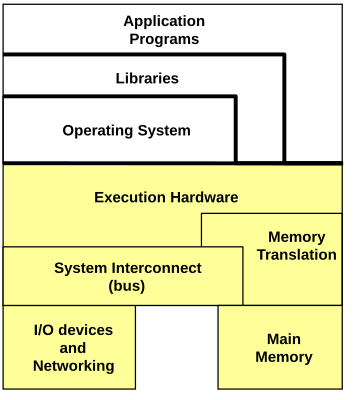
\includegraphics[width=.4\textwidth]{figures/MachineOS.png}
		\item Compiler developer
		\begin{itemize}
			\item Application Binary Interface (ABI)
			\item User ISA + OS calls
		\end{itemize}
		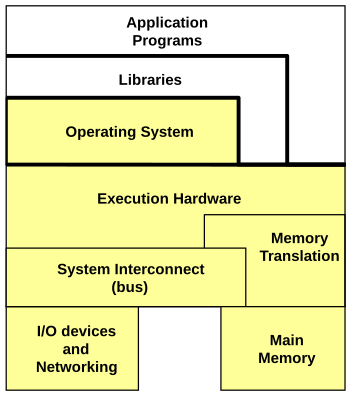
\includegraphics[width=.4\textwidth]{figures/MachineCompiler.png}
		\item Application programmer
		\begin{itemize}
			\item Application Program Interface (API)
			\item User ISA + library calls
		\end{itemize}
		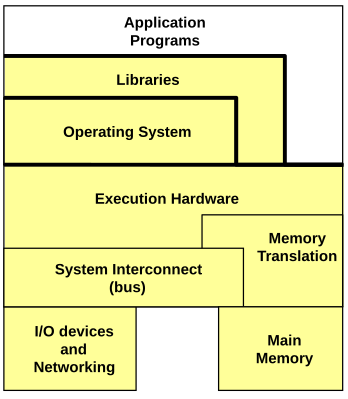
\includegraphics[width=.4\textwidth]{figures/MachineApplication.png}
	\end{itemize}
\end{itemize}

\subsection{Virtual Machines}

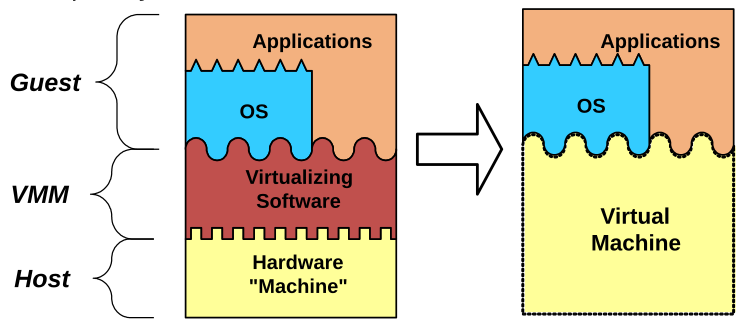
\includegraphics[width=.8\textwidth]{figures/VirtualMachines.png}

\end{document}